The theoretical predictions for the investigated signal processes are described in this sub-section. 
For each mass point available from the generated Monte-Carlo samples, cross sections are evaluated in the relevant parameter-space of the investigated benchmark models.  

The benchmark model we will consider is 2HDM type~II. This model is an ``MSSM-like'' model, in which one Higgs doublet couples to up-type quarks
and the other to down-type quarks and charged leptons. Another common choice from literature is the 2HDM type~I model, but type~I and 
type~II models only differ for their couplings to down-type fermions, thus they predict same cross sections for \ttH\ and \ttA. 

All used cross-sections for heavy neutral Higgs-bosons production are obtained from the standard HBSM recommendations \\
{\small{https://twiki.cern.ch/twiki/bin/viewauth/AtlasProtected/HiggsBSM2HDMRecommendations}} \\
from the LHC HXSG (Higgs Cross-Section working Group). The used version of the cross-sections is 1.6.6\_13TeV; in this version the default cross-sections are derived in the Santander matched 4FS+5FS scheme.

The cross sections in the alignment limit are presented in Fig.~\ref{fig:bench_xsec_ttH_1D}.

\begin{figure}[tbp]
	\begin{center}\setlength{\tabcolsep}{2.0pt}\small   

		\begin{tabular}{cc}
					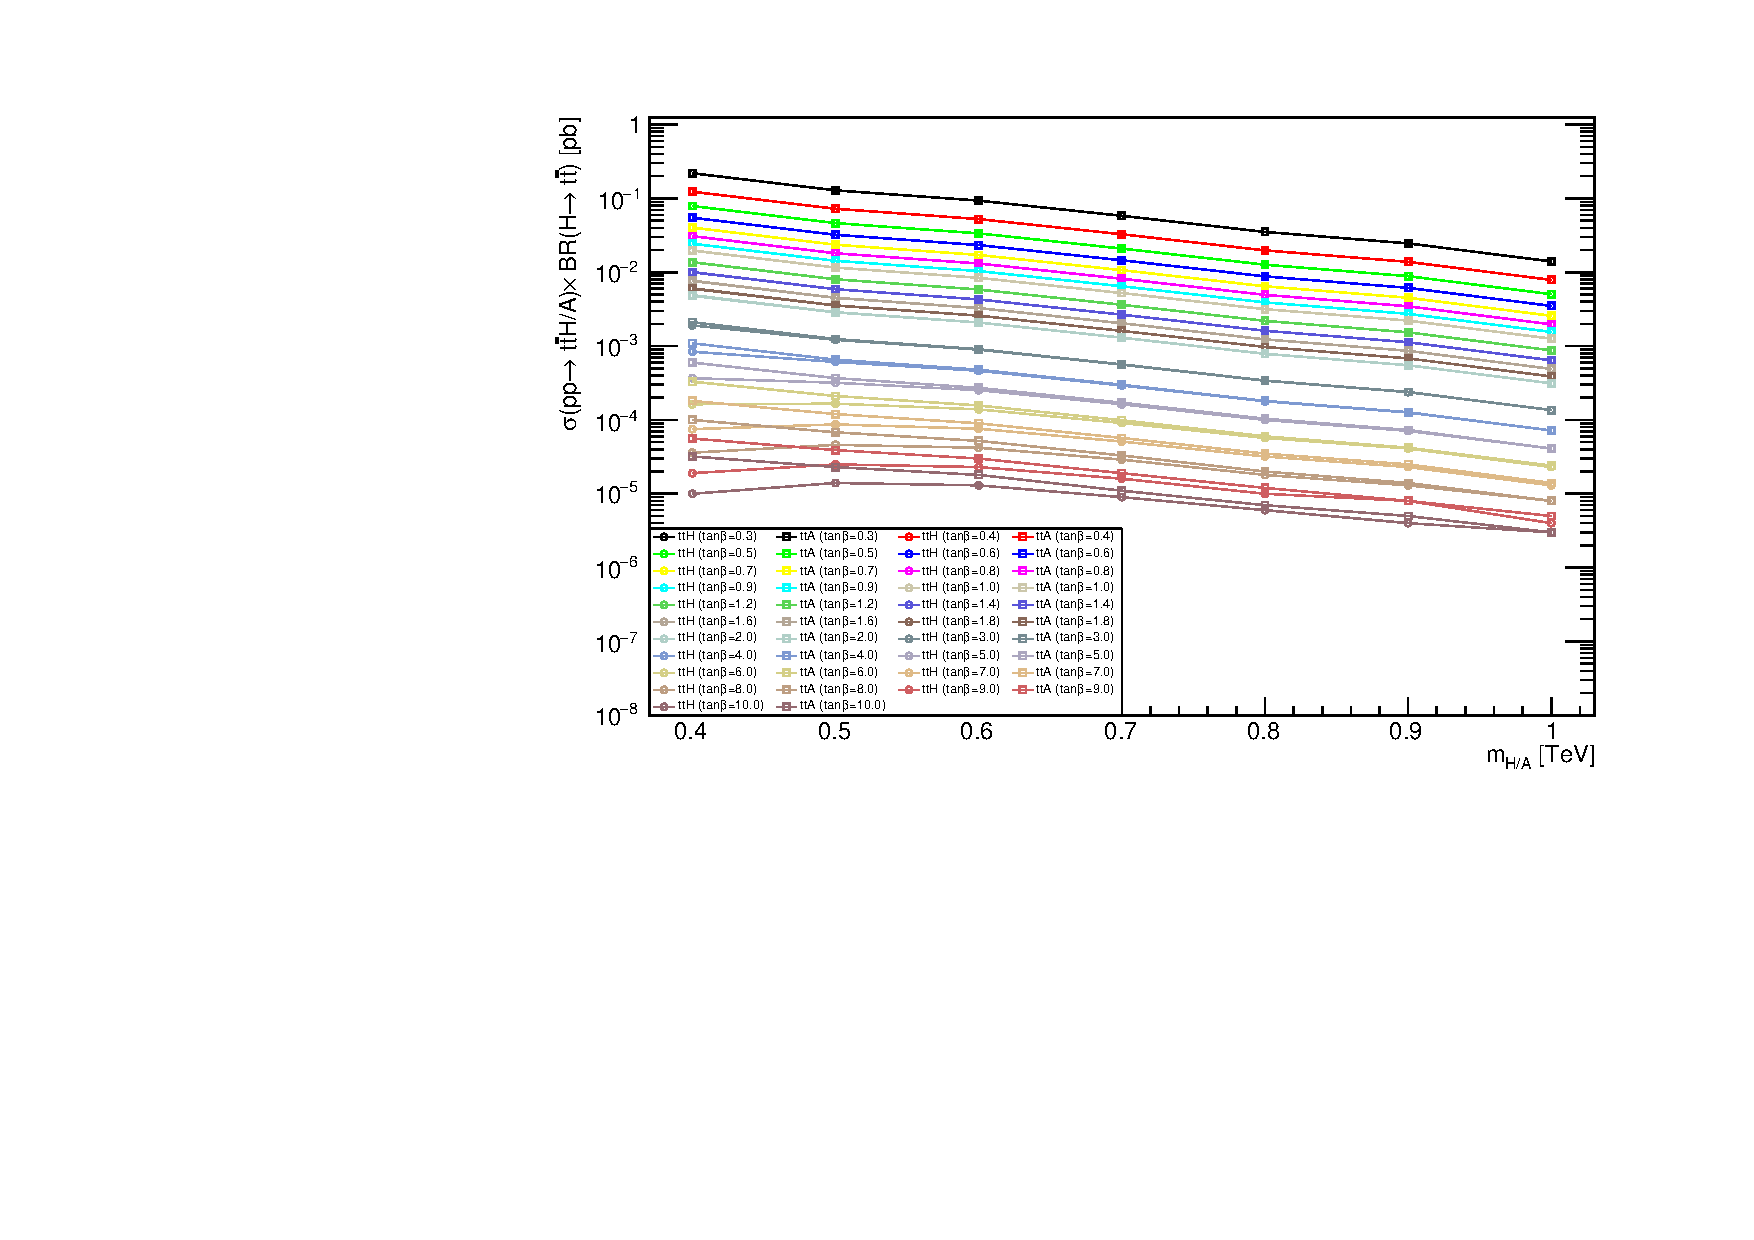
\includegraphics[width=0.47\textwidth]{figures/signal_modeling/hbsm_cross_sections/tanb_mass} 
					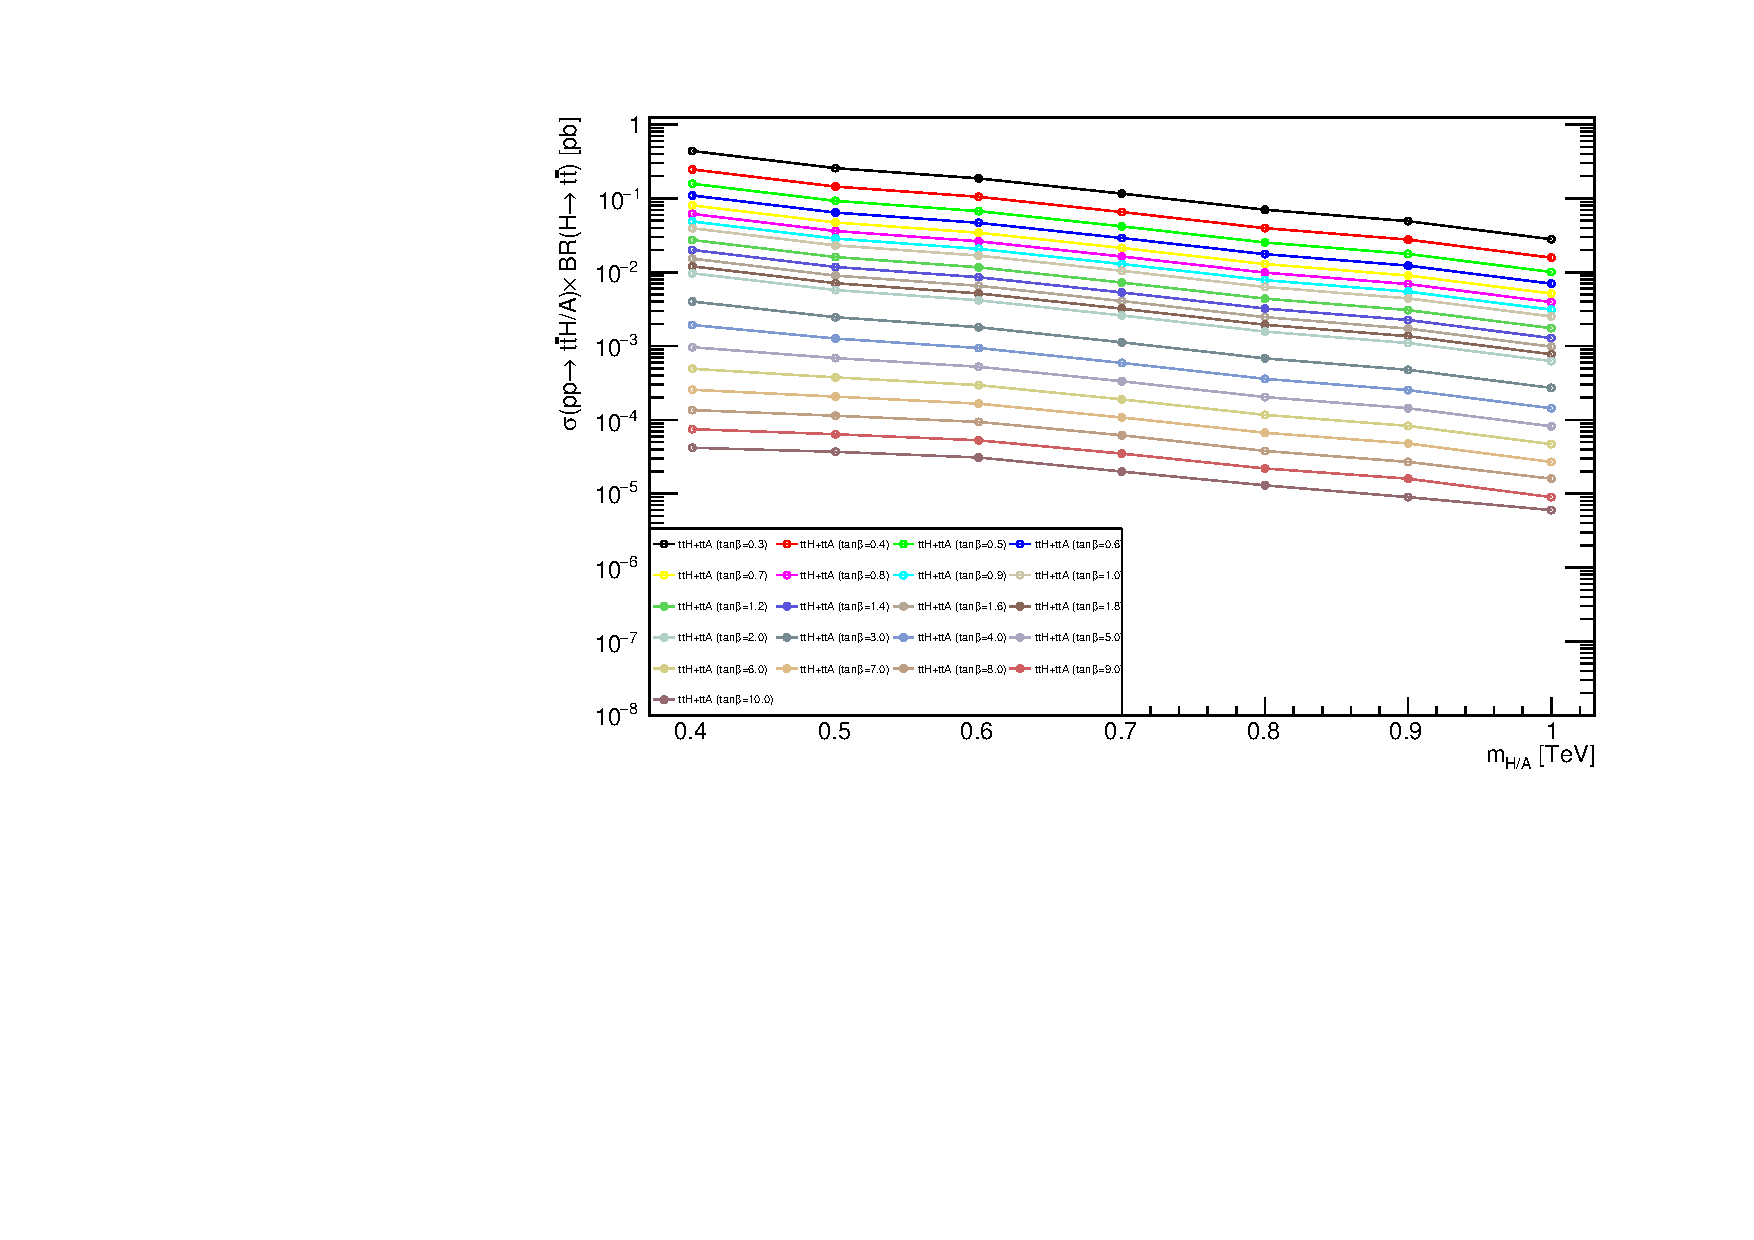
\includegraphics[width=0.47\textwidth]{figures/signal_modeling/hbsm_cross_sections/tanb_mass_merge_ttA_ttH} 
		\end{tabular}
		\caption{Cross-sections times branching-ratios for \ttH\ (left, circle marker), \ttA\ (left, square marker) and $\ensuremath{t\bar{t}H}+\ensuremath{t\bar{t}A}\rightarrow t\bar{t}t\bar{t}$\ (right, circle marker) in 2HDM type~II presented as a funtion of $m_{A}$ for several $\tan\beta$ points in the alignment limit.}
		\label{fig:bench_xsec_ttH_1D}
	\end{center}
\end{figure}
